\section{Una de un certamen antiguo -PyDI - Pregunta 2 C3 2014-2 CC CSJ}
La PyDI ha solicitado ayuda a los alumnos de IWI-131 para el desarrollo de algunas funciones que le permitan realizar búsquedas de comportamiento sospechoso de los ciudadanos de Pytonia.
\\
Para resolver esta tarea debes identificar a los posibles sospechosos para la PyDI, quienes siempre son \textbf{menores de 41 años} y publican en un medio \textbf{distinto de Twitter}. Para esto se revisan dos archivos, un con la información de los ciudadanos y otro con las publicaciones de los usuarios. Ejemplos de estos archivos y su formato son \texttt{publicaciones.txt} y \texttt{personas.txt}.
\\
En el archivo de publicaciones se tiene el rut del sospechoso y el medio en el cual fue publicado. En el archivo de personas se encuentra el rut, la edad y 3 calificaciones (valores enteros) relacionadas al nivel de amenaza de sus últimas 3 detenciones por la PyDI.
\\
Por último se tiene un archivo por persona con los mensajes enviados (sin puntuación), el nombre de estos es el rut de cada quien (Ejemplo el rut 15740994-7 tiene asociado el archivo \texttt{15740994-7.txt}).
\\Los siguientes archivos son un ejemplo de lo anterior

\begin{figure}[h]
    \centering
    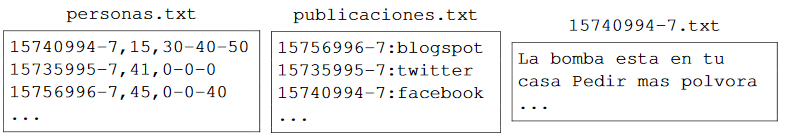
\includegraphics[width=\textwidth]{Guia/terroristas.png}
\end{figure}

Se le solicita a usted desarrollar las siguientes funciones:
\begin{itemize}
    \item[a.] Escriba la función \texttt{sospechosos(personas, publicaciones)} la cual reciba como parámetros dos archivos del tipo \texttt{personas.txt} y \texttt{publicaciones.txt}. Esta función debe retornar una \textbf{lista} con los rut de las personas que resulten sospechosas.
\begin{lstlisting}[style=consola]
>>> [*sospechosos('personas.txt','publicaciones.txt')*]
['15740994-7']
\end{lstlisting}
\item[b.]Escriba la función \texttt{leer\_mensajes(personas,publicaciones,claves)}, la cual recibe como parámetros 2 archivos del tipo \texttt{personas.txt} y \texttt{publicaciones.txt}, y una lista de palabras clave. Esta función debe retornar un diccionario cuya clave sea el rut de un sospechoso y el valor la cantidad de palabras claves que fueron encontradas en sus mensajes.
\begin{lstlisting}[style=consola]
>>> [*claves=['bomba','polvora','TNT']*]
>>> [*leer_mensajes('personas.txt','publicaciones.txt',claves)*]
{'15740994-7': 2}
\end{lstlisting}
\item[c.] Escriba la función \texttt{peligro(persona,publicaciones,claves)}, la cual recibe como parámetros 2 archivos del tipo \texttt{personas.txt} y \texttt{publicaciones.txt} y una lista de palabras clave. Esta función retorna una lista con los rut de los sospechosos considerados peligrosos. Un sospechoso es considerado peligroso si posee un ranking de peligrosidad mayor o igual a 30 y además posee al menos 2 palabras claves en sus mensajes. Donde el ranking de peligrosidad se determina promediando las 3 últimas palabras claves en sus mensajes. Donde el ranking de peligrosidad se determina promediando las 3 últimas calificaciones de detención.
\begin{lstlisting}[style=consola]
>>> [*claves=['bomba','polvora','TNT']*]
>>> [*peligro('personas.txt','publicaciones.txt',claves)*]
['15740994-7']
\end{lstlisting}
\end{itemize}